\section{Vorwort}
\hspace{0.5cm} Hallo!\\
Raus aus der Schule und rein ins Vergnügen. Nach 12 Jahren
langweiligen Deutschunterrichts und unzähligen Sozialkundestunden habt ihr es nun geschafft, an die Schwelle der unendlich hohen Treppe der Wissenschaft vorzuschreiten.\\
Ein neuer Lebensabschnitt der Arbeit, Verzweiflung, Frustration, aber auch der Freude liegt nun direkt vor euch und die Furien an euren Fü\ss en warten schon darauf, euch in ihren Bann des ewigen Wahnsinns zu ziehen.\\
Noch liegt all dies zwar in der Zukunft, aber wie immer schreitet die Zeit voran wie ein gro\ss er gekoppelter harmonischer Oszillator ohne Randbedingungen. Und wenn ihr heute noch lachen könnt über die üblichen
bösen Kommentare zu eurem Studium, wie z.B. von der amüsierten
Mutter: \enquote{Ein bisschen Studieren und abends Party machen\ldots}, so wird sich doch diese Meinung in der nächsten Zeit wandeln. Denn um es zusammenzufassen, habt ihr nun ASS und das steht nicht für ein Erkältungsmittel sondern für Arbeit, Stress und nochmal Stress. Also genießt nochmal das letzte freie Bier eures Lebens und auf in die Schlacht\ldots
\begin{figure}[b!]
	\centering
  	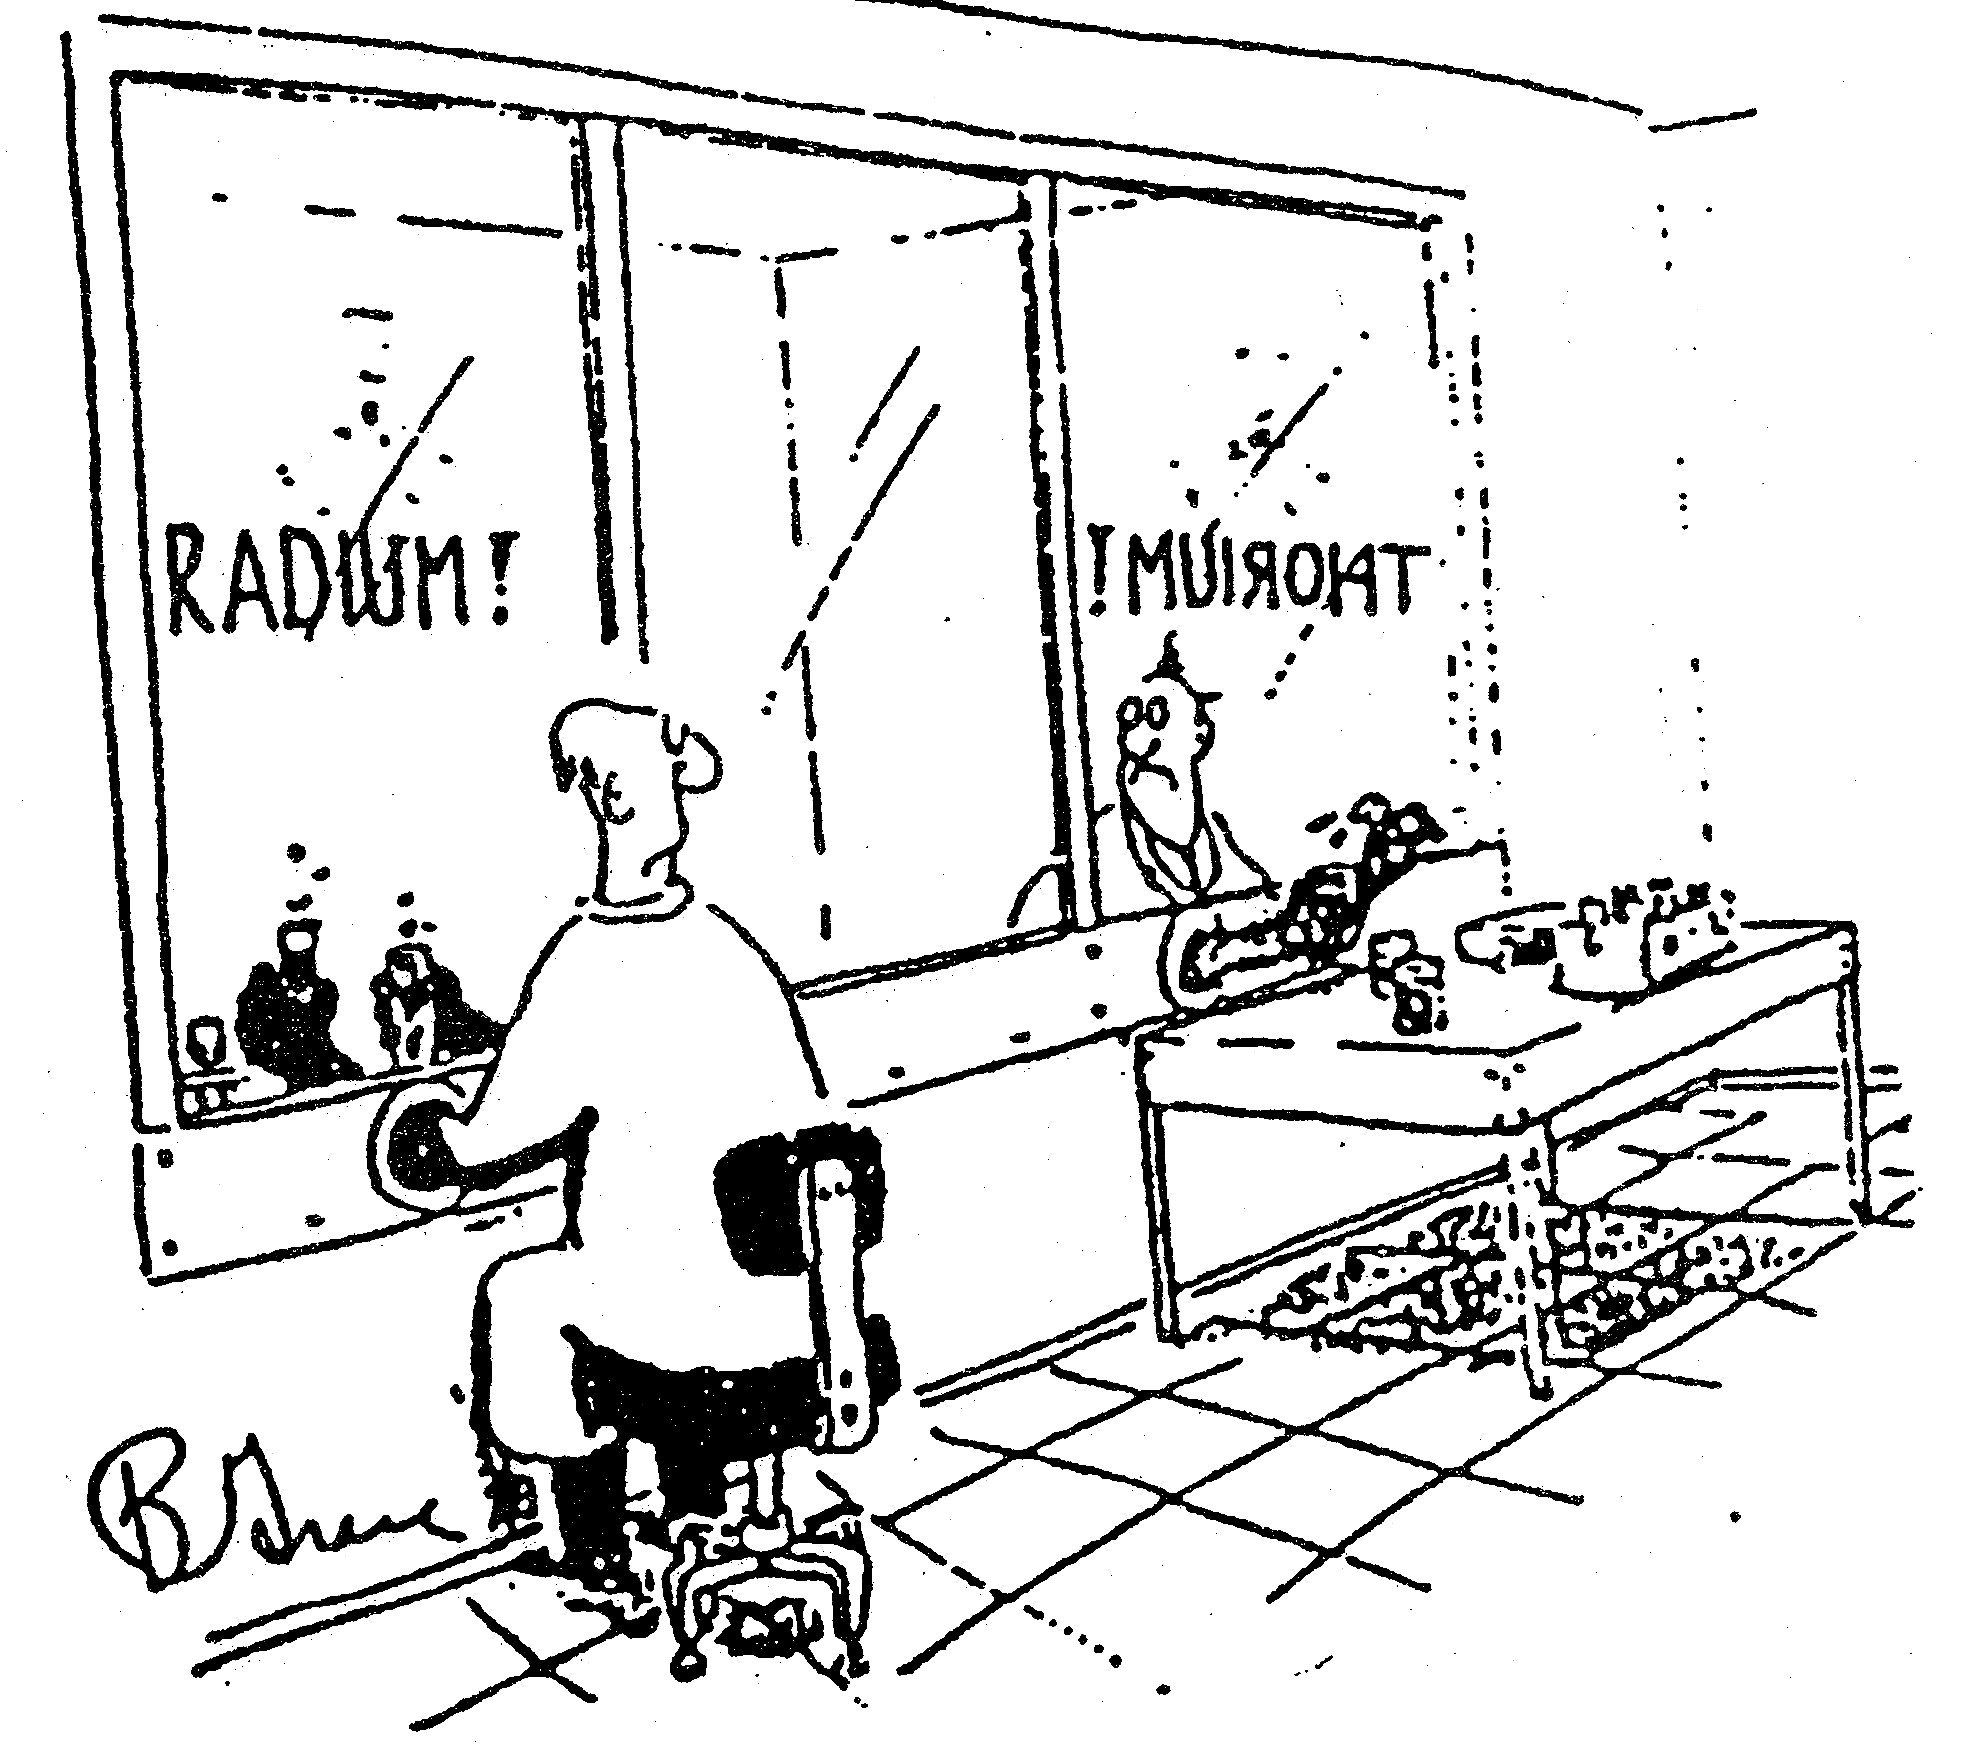
\includegraphics[width=.45\textwidth]{\imgdir/radium-thorium.jpg}
\end{figure}
\\So, das war nun die \enquote{Das-Leben-ist-ungerecht-und-alles-ist-so-schwer-Seite}. Aber zum Glück gibt es da ja noch die \enquote{Physik-ist-toll-Seite}. Und diese überwiegt definitiv die andere, da ihr euch das beste, interessanteste und umfassenste Studienfach ausgesucht habt, das es gibt.\\
Denn wenige Biologen werden euch erklären können, was ein Photon ist, noch weniger Chemiker, wie Quantenmechanik funktioniert, fast kein BWLer, wie man rechnet, und kein Jurist, wie man Partys feiert.\\
Also schätzt euch glücklich. Und auf den Spruch: \enquote{Physiker haben doch keine Freunde} könnt ihr bald getrost antworten: \enquote{Doch! Und zwar verdammt viele andere Physiker.}\\
In diesem Sinne: \textbf{Herzlich Willkommen} in der Physik!